\documentclass[12pt]{article}

\usepackage{fullpage}
\usepackage{graphicx}
\usepackage{hyperref}
\usepackage{listings}
\usepackage{multirow}
\usepackage{pdflscape}

\usepackage{glossaries}
\newacronym{doj}{US DOJ}{United States Department of Justice}
\newacronym{fps}{FPS}{Frames Per Second}
\newacronym{gps}{GPS}{Global Positioning System}
\newacronym{pcb}{PCB}{Printed Circuit Board}
\newacronym{sd}{SD}{Secure Digital}
\newacronym{tqfp}{TQFP}{Thin Quad Flat Package}
\newacronym{udp}{UDP}{User Datagram Protocol}
\newacronym{usb}{USB}{Universal Serial Bus}
\newacronym{uvc}{UVC}{USB Video Class}

\makeglossaries

\begin{document}

\setcounter{secnumdepth}{1}
\setcounter{tocdepth}{2}

\title{
\includegraphics[height=0.3\textheight]{logo}}
\date{}
\maketitle

\vfill

\begin{center}
    {\large EECS 473 - Advanced Embedded Systems - F15}

    \vspace{2.0em}

    \begin{tabular}{lr}
        Yun Chan Han & \url{ychani@umich.edu}\\
        Jiqing Jiang & \url{jqjiang@umich.edu}\\
        Alex LaBerge & \url{alaberge@umich.edu}\\
        Jacob Perrin & \url{tcperrin@umich.edu}\\
        Alec Ten Harmsel & \url{talec@umich.edu}\\
    \end{tabular}
\end{center}

\thispagestyle{empty}
\newpage

\tableofcontents
\thispagestyle{empty}
\newpage

\setcounter{page}{1}

\section{Overview}
Police officers around the country are beginning to wear body cameras to ensure
the safety of both themselves and the public. However, current body camera
solutions poorly manage the tradeoff between safety and privacy. To manage this
tradeoff, the \gls{doj} has asked law enforcement agencies to construct and
pilot programs for testing\cite{officer_privacy}.  Our product attempts to ease
policy concerns by creating a body camera system which intelligently decides
when to record footage by using various triggers, including environmental
stimuli and manual control.  Our project can be deemed a success in the sense
that we demonstrated a proof of concept. Our team created a police body camera
that decides to record based on the firearm being unholstered, loud noises, or
an officer controlled manual switch.  The quality of the recording was not
quite what we had been hoping for, but given the hardware we chose, we believe
that we could not have provided a much better final product. 

\begin{figure}[h]
    \centering
    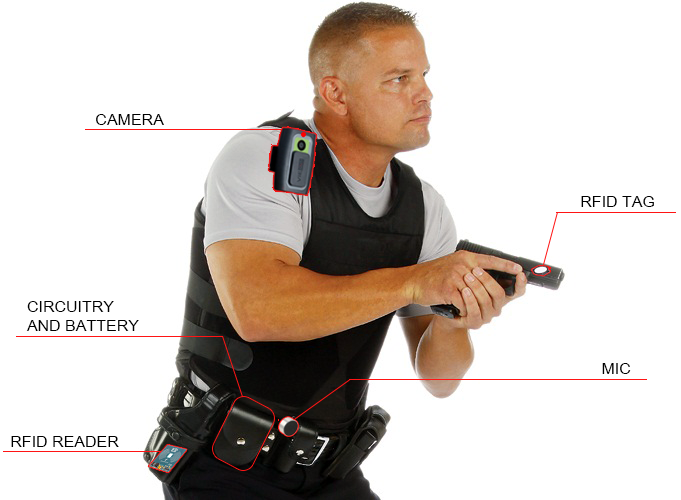
\includegraphics[width=0.9\textwidth]{installation}
    \caption{Overview of Installation}
    \label{fig:installation}
\end{figure}

At the design expo, we demonstrated our project (physical layout shown in
Figure \ref{fig:installation}).  Our project is a self-contained, enclosed
product which wirelessly sends camera footage to a laptop at about 1 \gls{fps}.
The product saved camera footage to a \gls{sd} card at a more reasonable 10
\gls{fps}.  The success of this project was in question until nearly the very
end, due to the fact that the \gls{usb} protocol driver was a much heartier
challenge than originally anticipated. The team met most other milestone
objectives with flying colors. Given this, and the fact that the final product
was what we had proposed (even with some weaker specifications), our project
should be deemed a success and we are happy with the result.

\section{Description}
Every year around 500 people are killed by law enforcement personnel, and many
people are wondering how many of these deaths were justified. One classic way
to ensure that all protocols were being followed has been a police body camera.
However, these are often expensive (\$800 - \$1200 each\cite{cam}) and have
serious privacy concerns for the police officers. If the body cameras are
always on, it might record personal moments that do not need to be seen.
However, if we give the officer a way to turn it on and off, police may tamper
with evidence that could convict them. Benson discusses the various incentives
at work that determine which arrests police are likely to
make\cite[ch.~6]{enterprise_of_law}. Similarly, police have an incentive to use
their weapons to stay alive often since they are rarely prosecuted in cases in
which they use lethal force\cite{no_conviction_1,no_conviction_2}. This is not
to say that police officers are bad, but that they face incentives that can be
very strong and may override their sense of duty.

\subsection{Objectives}
When purchasing body cameras, police departments must analyze the costs and
benefits.  In addition to the high cost of current units\cite{cam}, storing the
amount of footage from body cameras that are always on represents a significant
challenge\cite{store1,store2}. Another dilemma facing current solutions is how
to deal with respecting the privacy of the officer\cite{officer_privacy}. Our
product meets the above objectives by being below the current average cost and
by only recording footage of violent situations. In addition, our product meets
objectives relating to safety and legal liability.  To increase safety, backup
may be automatically dispatched when our product signals violence before the
officer has time to call for it. To minimize legal liability and reduce the
likelihood of corruption, a police department may purchase third-party
streaming attachments to stream video\footnote{We have not seen any articles on
    reducing liability applied to this topic, but contracting liability to a
third party is commonly done in business.}.

\subsection{System Description}

\begin{figure}[h]
    \centering
    \includegraphics[height=0.35\textheight]{sys_desc}
    \caption{High level system design}
    \label{fig:system_description}
\end{figure}

Our project can be easily broken down into two systems: a trigger system and a
record system. A functional block diagram of these systems and their related
subsystems is shown in Figure \ref{fig:system_description}. The trigger system
serves as a ``trigger'' to wake up the record system when the system senses a
potentially violent situation. The MSP430 contains code which determines when
the Tiva should be awoken based on selected events. When the MSP430 decides
that an event should be recorded, it sends a signal to the Tiva, which serves
as an interrupt to wake up the larger processor. This same signal also toggles
a set of MOSFETs which control power to the record system related peripherals.
Together, these two systems make up a product which can be smarter and lower
power than current solutions.

\subsection{Trigger System}
\label{sec:sys_trigger}

\begin{figure}[h]
    \centering
    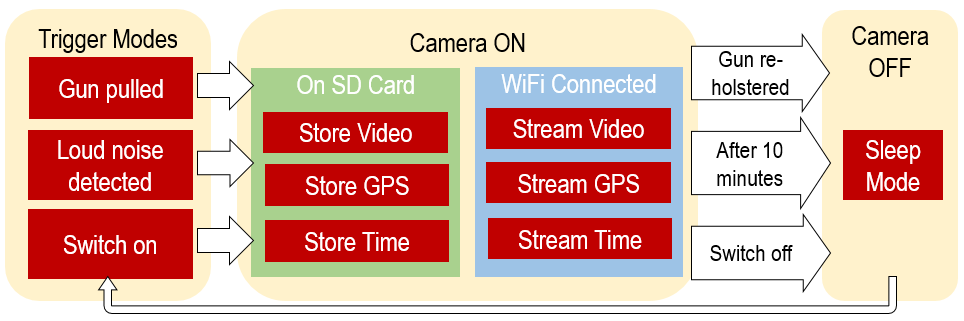
\includegraphics[width=0.9\textwidth]{trigger_flow}
    \caption{Trigger flow}
    \label{fig:trigger_flow}
\end{figure}

The trigger subsystem, shown in Figure \ref{fig:trigger_flow}, consists of the
hardware and software used to process our triggers and send an interrupt to the
Tiva to begin or end recording. The MSP430 takes in a comparator line that
determines the microphone level, an \gls{rfid} radio card present line, and a
manual switch and determines when to wake the Tiva based on those inputs.

We chose the MSP430 because it is a very low power processor that has enough
GPIO pins to fit our need. When not receiving interrupts off of the 3 trigger
lines, it is put into a low power mode with interrupts enabled, which allows
minimal current draw while maintaining full functionality.

The most important trigger for this project is the \gls{rfid} radio. We use the
ID-12LA \gls{rfid} radio because it is relatively low power and matched the
frequency of the sticker tags we wanted to use. It has a ``Card Present'' line
which is high when a tag is present and low when there is no tag, which
simplified the interface for this part greatly. \gls{rfid} tags also work on
metal, allowing integration with typical officer sidearms.

We use a switch on the device in order to allow the officer to turn on the
device if he feels unsafe. However, the switch cannot turn off the device if
any of the other triggers are present. 

The microphone input is calibrated with two on-board potentiometers,
controlling gain and triggering threshold, that can be customized for an
officers environment. This value is then put into an analog comparator that
triggers an MSP430 interrupt when the microphone value has surpassed the
threshold value. The trigger is high for 10 minutes after a microphone event,
which is controlled by a timer on the MSP430.

Mechanically, many of these triggering mechanisms are located outside of the
enclosure. This allows for little interference between the enclosure and the
\gls{rfid} radio. This also allows the user to be able to easily access the
switch and the microphone to be able to pick up smaller sounds.

\subsection{Record System}
\label{sec:sys_video}
The record system consists of the hardware and software used to capture video
from a source and send it to various sinks. The source of the video is any
camera that complies with the \gls{uvc} standard. There are currently two
implemented sinks: an on-board \gls{sd} card and streaming to a base station
over Wi-Fi. The larger of the two onboard processors, a Tiva, manages the
transfer of video from source to sinks. The flow of video through the system is
shown in Figure \ref{fig:video_flow}.

\begin{figure}[h]
    \centering
    \includegraphics[width=0.9\textwidth]{subsys_video}
    \caption{Video subsystem}
    \label{fig:video_flow}
\end{figure}

Currently, the driver that handles the video source is compatible with and aims
to fully comply with versions 1.1 and 1.5 of the \gls{uvc}
standard\cite{uvc_standard_11,uvc_standard_15}. The driver supports both a raw
video format\footnote{Specifically the YUY2 encoding} and the MJPEG format. In
order to obtain the highest-quality video at the lowest bandwidth, the driver
prefers MJPEG over raw. In order to choose a resolution, the driver is
initialized with a target bandwidth and then chooses a frame size that will be
as close to that bandwidth as possible without exceeding it. Due to the
limitations of the Wi-Fi hardware, a frame size of 160 x 120 is the largest
resolution that can be streamed. The driver initialization function declaration
is shown in Appendix \ref{app:software_interfaces}.

The Tiva processor is triggered on by the trigger system, which is described in
Section \ref{sec:sys_trigger}. Once triggered, the Tiva wakes from sleep and
opens connections to the attached camera, the on-board \gls{sd} card, and the
base station via the Wi-Fi chip. As video data flows in from the camera, the
\gls{uvc} driver uses callbacks to announce the start of a frame, the data in a
frame, and the end of a frame. Using those callbacks, the video data is both
written to the \gls{sd} card and streamed to the base station. The Tiva
processor does not run an operating system, decreasing its response time and
increasing its performance.

Our SD card writer is a modified SPI driver that runs through a library called
FatFS. This formats the SPI messages to open files and write to those files
with relative ease. Our implementation takes the frame that is received from
the USB and writes it to a file in plaintext. From there we can use a similar
implementation on our base station as the WiFi receiver to display the frames
with a small delay inbetween to simulate frame rate. 

The Wi-Fi streaming is comprised of two components: a CC3000 chip that handles
the wireless connection on the body camera system and a base station that runs
on a computer. The CC3000, using the \gls{udp} protocol-based proprietary
packet format shown in Table \ref{tab:packet_format}, streams video data to the
base station.  The base station receives the video packets, combines the
various chunks in the correct order, saves to a hard drive, and displays the
video on-screen.

\begin{table}[h]
    \centering
    \caption{Body Camera Streaming Protocol}
    \vspace{1.0em}
    \begin{tabular}{lrr}
        \textbf{Field} & \textbf{Offset} & \textbf{Size (bytes)}\\
        length & 0 & 2\\
        ID & 2 & 1\\
        type & 3 & 1\\
        offset & 4 & 4\\
        data & 8 & length\\
    \end{tabular}
    \label{tab:packet_format}
\end{table}

By saving locally, our product provides resiliency. When a network is not
available, all video data is still saved. It is impossible to destroy the
evidence by jamming the wireless network signal, so even extremely resourceful
criminals and/or very electrically noisy environments will not prevent evidence
from being gathered. By streaming data to a police department or third party
network, our product increases the immediate safety of all parties involved and
provides redundancy to reduce the chance of evidence destruction. The safety of
the parties involved in a violent situation is increased because the police
department knows as soon as an officer enters a violent situation. Backup may
be dispatched without the officer having to request it; in cases where an
officer unknowingly walks into a dangerous situation, this feature is
life-saving.

\subsection{Power System}
Our system is designed to use as little energy as possible by removing power to
all video-related subsystems until video needs to be recorded. The video
subsystem consists of a Texas Instruments Tiva
microcontroller\cite[p.~1880]{tm4c1294ncpdt}, a Texas Instruments CC3000 Wi-Fi
chip\cite[p.~6]{cc3000}, an SD card\cite[p.~19,23]{sd_standard}, a EM-506 \gls{gps}
unit\cite[p.~10]{em506}, and a USB camera\cite[p.~245]{usb_standard}. These
parts draw the vast majority of the power, totalling 4290.4 mW in the worst case.
The rest of the system, composed mostly of the trigger system, draws a relatively small 131.4 mW. The individual worst
case power draws are given in Table \ref{tab:worst_case_power}.

\begin{table}[h!]
    \centering
    \caption{Worst Case Power Consumption}
    \vspace{1.0em}
    \begin{tabular}{lrrr}
        \textbf{Device} & \textbf{Voltage (V)} & \textbf{Current (mA)} & \textbf{Power (mW)}\\
        Tiva & 3.3 & 133.4 & 440.2\\
        Camera & 5.0 & 500.0 & 2500.0\\
        GPS & 5.0 & 55.0 & 275.0\\
        Microphone & 3.3 & 0.5 & 1.0\\
        RFID Reader & 3.3 & 35.0 & 115.5\\
        SD Card & 3.3 & 100.0 & 330.0\\
        MSP430 & 3.3 & 4.5 & 14.9\\
        CC3000 & 3.6 & 207.0 & 745.2\\
        \hline
        \textbf{Totals} & & & \textbf{Power (mW)}\\
        Idle & & & 131.4\\
        Recording & & & 4421.8\\
    \end{tabular}
    \label{tab:worst_case_power}
\end{table}

Using a 25Wh battery, an officer can record for 1.5 hours. The battery may be
upgraded as needed, depending on the workload of the officer.

\subsection{Mechanical Design}

\begin{figure}[h]
    \centering
    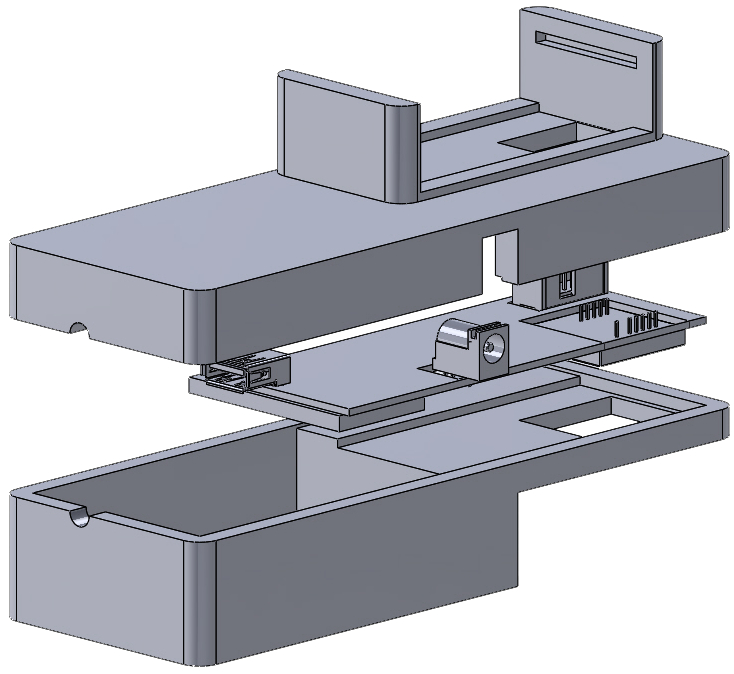
\includegraphics[height=0.35\textheight]{exploded_enclosure}
    \caption{Exploded view of enclosure with \gls{pcb}}
    \label{fig:exploded_enclosure}
\end{figure}

We made an enclosure that houses all the components except a battery and a
camera, shown in Figure \ref{fig:exploded_enclosure}. The enclosure was
intended to be tamperproof (or as tamperproof as possible for a prototype) by
preventing connections to a \gls{usb} camera and a \gls{sd} card from being
disconnected.  Due to the limitation of a 3D printer and the design of our
\gls{pcb}, the enclosure design was not the most optimal, wasting a lot of
space inside the enclosure.  The enclosure is attached to the holster and had
an opening at the bottom to minimize the distance between the \gls{rfid} reader
and a \gls{rfid} tag on the firearm.  This ensures an accurate detection of the
state of the firearm - whether it is holstered or otherwise. If this project
were to be moved towards production, the product would need considerable
improvement in the area of the enclosure, but since we are not skilled in this
area, we feel that the current state is more than satisfactory. The enclosure
has a mass of 209 grams, and has dimensions of 166 x 62 x 24mm.

The \gls{usb} camera was mounted on the shoulder of the officer. Since most
police officer uniforms have a shoulder strap, USB cameras with clips can be
easily mounted. However, this can be improved by designing our own camera mount
so that any camera can be firmly mounted on the shoulder without any external
clips. In addition, a more secured mount would be optimal to improve video
quality and directionality.

\section{Milestones, Schedule, and Budget}
Most of this project was on schedule from the beginning. The only problem we
really ran into was getting our final piece of the puzzle in place: decoding
our video. Once that was working, the remainder of the project was quickly
integrated and a full feature prototype was able to be tested. Our original
schedule is shown in Appendix \ref{app:gantt}. All deadlines were met except
for the Camera Driver, which was not in testing until late November and not
finished until early December.

Our original budget was around \$312.93 and we spent \$884.91.

\subsection{Milestone 1}
\subsubsection{GPS and RTC Implementation and Verification}
Getting an early \gls{gps} parser was one of the easier parts of the project.
It was also one of the more unnecessary parts for a working demo. \gls{gps} was
done early, but it turned out not to be very vital to the success of the
project.

\subsubsection{Audio and Manual Trigger Implementation and Verification}
Quickly getting this system prototyped was a very early victory that helped the
trigger side of our project get done as quickly as it did. We had a working
prototype for the MSP430 trigger processor about a week before the first
milestone and we had a final version a few weeks later, which ensured that once
we got all of the Tiva video processing done, we could easily integrate the two
parts together.

\subsubsection{Wi-Fi Testing}
Originally we had a UART-based WiFi module that did not have thorough
documentation or any sort of support on the internet. With this in mind, and
the fact that it seemed to overheat easily, we looked for a quick replacement.
What we found was the CC3000, which boasted a 4Mbps data transfer rate over
TCP.  Having a little bit of background in networking, we figured UDP would be
even faster so we locked this in as our choice and quickly had a demo in which
we sent packets over to a host computer.

\subsubsection{RFID in Development}
We managed to find a reliable \gls{rfid} radio that had a tag-present line
which suited our needs very well. The development on this part was basically
nonexistent, and thus the trigger processing reached completion even quicker.
We had the \gls{rfid} component completely working by the time this milestone
came around.

\subsubsection{Video Data Encoded}
Video data was the slowest part of our project to develop, since writing a
\gls{usb} device driver was no small task. We did not manage to see video until
around a month and a half after the first milestone. This milestone portrayed
both our hearty ambition and innocent ignorance.

\subsection{Milestone 2}
\subsubsection{Working Full-Featured Prototype}
This was definitely the issue that kept us behind on our project. We did not
have verified data by the second milestone, so it was difficult to test
anything. Our team had all of the other parts done (i.e. a WiFi driver that
could send at a reasonable speed and all of the trigger processing in its final
state), but without being able to see video we were not sure whether or not the
project would be completed on time.

\subsubsection{PCB is Shipped}
We overestimated the time required to get a \gls{pcb} out, so by the time the
second milestone came around we had already populated our \gls{pcb} and begun
testing.  Luckily for us, we had plenty of time to order a second version of a
\gls{pcb} which addressed problems we had such as an incorrect crystal, an
unorderable \gls{sd} card reader, and a few small on-board revisions we needed
to make. Getting this done as early as we did definitely helped us stay on
track.

\subsubsection{Enclosure Designed}
Designing the enclosure also took less time than anticipated. Our team had a
first version enclosure printed that helped us form the next and final version
that we have on the final prototype. Having this milestone completed also
helped us stay on track.

\section{Lessons Learned}
When we reflect on the outcome of our project, there are a few points that we
wish we would have known before the project started.

The first mistake our group made was to create specifications and requirements
without first researching to a point where we would be able to realistically
quantify them. Instead, we had a tendency to create requirements based on the
ideal case - what we thought would be nice to have or a good goal to have. This
lack of research is reflected in the part choices we made (i.e. the CC3000),
and really propagated throughout our entire project. The common saying
``measure twice, cut once'' comes to mind with regards to this situation.

Also, we learned that most tasks require steep learning curve, and it is very
hard for other members to participate in tasks that have already made
significant progress. Other members found it difficult to help with incomplete
tasks after completing their given tasks. Time was limited for the original
member of the task to walk through the progress that he had already made. This
resulted in some of team members doing more work than the others. We learned
that it is important to distribute work correctly and that all team members
keep track of each other's tasks.

An element of our project that really went well was the choice of development
board and process we used to convert our development platform to a custom
\gls{pcb}.  The development board had a great deal of pinouts and functionality
that made the schematic creation process easy. We were able to test on the
development board using the exact same pins and peripherals that would later be
used on the PCB. This meant that once the hardware was ready and correct, the
software worked almost immediately, with little software debugging.

The design of the enclosure was an afterthought, and the project appeared to be
poorly integrated because of this. The enclosure was bright blue, and very
noticeably duct-taped to the officer's holster during the design expo. Another
reason for the poor enclosure design was that the PCB was routed with the sole
constraint that it should work, and no thought was given to a good form factor
for packaging. In the future, care should be taken to route the circuit
board(s) in such as way as to integrate well with the officer's belt and
holster.

Overall, if we could send a message to ourselves before the project started, it
would be to continue to work hard from the beginning and to not underestimate
the complexity from USB. Our group did a great job working a steady,
substantial amount throughout the life of the project. We did end up having to
work more towards the end of the project, but this was because we had
underestimated the amount of work the USB driver would require, and this
delayed all parts, including work on the PCB. So, if we could go back and
increase work on this portion of our project in the beginning, or avoid
undertaking that monstrous task altogether, we feel that this project would
have been less stressful and more successful.

\subsection{Individual Lessons Learned}
Alec learned about writing a USB device driver, and choosing video formats
based on bandwidth constraints. He also experienced soldering a TQFP with more
than 64 pins for the first time, and learned from Yitian how to use flux to fix
solder bridges. He also learned a bit about designing a network protocol.

Alex learned about researching parts. This involved not only finding a part
that meets the requirements of the project, but also researching different
sources for the same part. This was learned the hard way by choosing a WiFi
module that has been retired and is no longer supported by TI, something that
made finding resources much more difficult. He also learned about PCB
verification and how to make sure individual parts of the PCB are working while
not having the others functional. 

Jacob learned about designing a PCB using Eagle. This involved coordination
with each team member to discuss options regarding schematic (pin selection)
and layout considerations. After fabrication, he was forced to learn a great
deal about debugging hardware, including what not to do (i.e. shorting pins
with bad probes).

Jiqing got familiar with the process of programming in Code Composer Studio
from TI and 3D design by using Solidworks. He learned about reading from and
writing to an \gls{sd} card via SPI communication and how each individual
function got integrated in a whole system. He also learned about using a Saleae
Logic Analyzer to debug and asking TI support team online for help. He worked
with Alec on establishing a \gls{usb} device driver in the beginning of the
project and learned how \gls{usb} works with the help of Alec and examples from
documents.

Yun learned about an overall real-application design process that includes
\gls{pcb} design and manufacturing, 3D design and printing, and group
coordination through GitHub. He learned how to implement microcontroller code
using Code Composer Studio, and designing 3D parts using Solidworks. Also, he
learned about video protocols and various encoding and decoding methods.

\section{Contributions}
A summary of individual contributions is given in Table
\ref{tab:individual_contrib}, and details are given below.

\begin{table}[h]
    \centering
    \caption{Individual team member contributions}
    \vspace{1.0em}
    \begin{tabular}{llr}
        \textbf{Team Member} & \textbf{Summary of Contribution} & \textbf{Effort}\\
        Alec Ten Harmsel & UVC driver, base station, power analysis & 25\%\\
        Alex LaBerge & Wi-Fi driver, \gls{gps}, sleep mode, \gls{pcb} verification & 25\%\\
        Jacob Perrin & \gls{pcb} design and assembly, group coordination & 20\%\\
        Jiqing Jiang & \gls{sd} card driver, \gls{uvc} driver, enclosure design, poster design & 15\%\\
        Yun Chan Han & Trigger circuitry/software, enclosure design, poster design & 15\%\\
    \end{tabular}
    \label{tab:individual_contrib}
\end{table}

Alec was responsible for the \gls{uvc} device driver. This driver parsed the
configuration of the connected \gls{usb} camera, determined the optimal format
and video size based on bandwidth constraints, and then configured the camera.
After camera configuration, the driver also implemented the “top” side of an
interrupt-based video capture solution. In addition, Alec wrote the base
station code, which listened on the network for video broadcasted by the body
camera system, converted it to a displayable format with OpenCV, and displayed
it with the Qt Toolkit. Finally, Alec was responsible for the power system
design and reviewing the circuit schematics and layouts produced by Jake.

Alex was responsible for the main control loop for the Tiva recording software,
which included integrating his WiFi and \gls{gps} drivers in with Alec's USB driver.
He debugged the SD card implementation and formatted Jiqing's driver to work with
the pins that the PCB used, as well as integrated that feature into the control loop. 
He optimized the TI library for the WiFi module to get the fastest throughput
possible on the CC3000 by removing unnecessary delays and making the sockets
nonblocking. Alex also wrote the first iteration of base station socket code
which received the data streamed from the Tiva, which was later improved by
Alec. Finally, Alex was responsible for verifying the components on the PCB
worked and debugging the issues that arose.

Jacob was primarily responsible for all activities related to the hardware, and
specifically the PCB. As such, he designed the schematic and layout for the
PCB. The PCB was designed before most parts of the prototype had been finished,
or even begun. As such, this took a good deal of effort and care (there are
still small errata on the current version of the PCB). He also took part in the
assembly of four different PCB boards. Additionally, Jacob was responsible for
coordinating group activities and communication with outside parties. This
includes getting sponsored by Advanced Circuits as well as doing any
miscellaneous grunt work that the group came across through the life of the
project.

Jiqing was responsible for the implementation of saving video data to a micro
\gls{sd} card and the enclosure design in Solidworks. He also helped to debug
during system integration and checking \gls{pcb} design when bugs were
discovered.  He also worked with Alec on the \gls{uvc} device driver and
designed the poster.

Yun was responsible for the hardware and software of the triggering portion of
the project. He designed the schematic of a circuitry that takes analog and
digital inputs from a switch, a microphone, and an \gls{rfid} reader. The
circuitry he designed was adjustable allowing the noise level can be controlled
externally.  He designed the triggering logic to start and end the video
recording on the MSP430. He also designed an enclosure that protects the
\gls{usb} cable connection and \gls{sd} card from users. He designed the poster
for design expo as well.

\section{Cost of Manufacture}
Our total estimated cost of manufacturing is \$120 for any quantity greater
than 150. This seems like a very reasonable number given the price of the parts
listed above. This quote includes the WiFi breakout and \gls{rfid} module. The
only additional pieces of hardware that would be needed in order to make this
quote a complete package would be the camera, battery, and enclosure. These
items would likely bring the price to manufacture this item to somewhere closer
to \$200-\$250. Given that we would need to rethink some partitions of this
project, most important among these being WiFi bandwidth and microprocessor
processing power, this number does appear to be very rough. However, with this
cost of manufacturing, such a product could be very competitive in this market,
where prices can often be found near the \$1000 range.

\section{Parts}
Our list of parts is shown in Tables \ref{tab:parts_1} and \ref{tab:parts_2}.

\begin{table}[h]
    \centering
    \caption{Part List: Part 1}
    \vspace{1.0em}
    \begin{tabular}{lrrrl}
        \textbf{Part} & \textbf{Unit Cost} & \textbf{Quantity} & \textbf{Total Cost} & \textbf{Model}\\
        Sticker RFID Tags & \$10.87 & 1 & \$10.87 & \href{http://www.amazon.com/gp/product/B00UGHPWZK?psc=1&redirect=true&ref\_=oh\_aui\_detailpage\_o00\_s00}{LockState LS-STPeel}\\
        USB Female Coupler & \$7.99 & 1 & \$7.99 & \href{http://www.amazon.com/gp/product/B00J4NMTMQ?psc=1&redirect=true&ref\_=oh\_aui\_detailpage\_o02\_s00}{USB 3.0 Female Coupler}\\
        Genius Webcam & \$39.21 & 1 & \$39.21 & \href{http://www.amazon.com/gp/product/B0080CE5M4?psc=1&redirect=true&ref\_=oh\_aui\_detailpage\_o05\_s00}{Genius WideCam F100}\\
        Belt Holster & \$9.49 & 1 & \$9.49 & \href{http://www.amazon.com/gp/product/B0018LA0UK?psc=1&redirect=true&ref\_=oh\_aui\_detailpage\_o07\_s00}{UTG Deluxe Commando Holster}\\
        SD Cards & \$10.65 & 1 & \$10.65 & \href{http://www.amazon.com/gp/product/B00FM5E1EY?psc=1&redirect=true&ref\_=oh\_aui\_detailpage\_o06\_s00}{SanDisk 8GB SD Card - 2 Pack}\\
        RFID Reader & \$49.95 & 1 & \$49.95 & \href{https://www.sparkfun.com/products/13198}{SparkFun RFID Starter Kit}\\
        CC3000 Wifi & \$34.95 & 1 & \$34.95 & \href{https://www.sparkfun.com/products/12072}{SparkFun CC3000 Breakout}\\
        PCB & \$33.00 & 2 & \$66.00 & \href{http://www.4pcb.com/}{http://www.4pcb.com/}\\
        TIVA C 1294 XL & \$19.99 & 1 & \$19.99 & \href{https://store.ti.com/tiva-connected-launchpad.aspx}{EK-TM4C1294XL}\\
        USB Connector & \$1.50 & 2 & \$3.00 & \href{https://www.sparkfun.com/products/437}{USB Male Type A Connector}\\
        SD socket & \$1.95 & 2 & \$3.90 & \href{https://www.sparkfun.com/products/12769}{SD/MMC Socket}\\
        Ribbon header & \$1.50 & 3 & \$4.50 & \href{https://www.sparkfun.com/products/8506}{2x5 Pin Shrouded Header}\\
        Ribbon Cable & \$1.50 & 1 & \$1.50 & \href{https://www.sparkfun.com/products/8535}{2x5 Pin IDC Ribbon Cable}\\
        Microphone & \$0.95 & 2 & \$1.90 & \href{https://www.sparkfun.com/products/8635}{Electret Microphone}\\
        Switch & \$0.75 & 2 & \$1.50 & \href{https://www.sparkfun.com/products/9609}{SPDT Slide Switch}\\
        LED & \$0.50 & 3 & \$1.50 & \href{https://www.sparkfun.com/products/10632}{Diffused LED - Red 10mm}\\
        TIVA Processor & \$16.95 & 2 & \$33.90 & \href{https://www.digikey.com/product-detail/en/TM4C1294NCPDTI3/296-38028-ND/4914951}{296-38028-ND}\\
        MSP430 Processor & \$2.46 & 2 & \$4.92 & \href{https://www.digikey.com/product-detail/en/MSP430G2553IPW20R/296-28430-1-ND/2638889}{296-28430-1-ND}\\
        MOSFETs & \$0.20 & 10 & \$1.95 & \href{https://www.digikey.com/product-detail/en/IRLML2402TRPBF/IRLML2402PBFCT-ND/812508}{IRLML2402PBFCT-ND}\\
        Crystal & \$0.79 & 2 & \$1.58 & \href{https://www.digikey.com/product-detail/en/403C11E16M00000/CTX732CT-ND/1638187}{CTX732CT-ND}\\
        LDO 3.3V & \$1.04 & 2 & \$2.08 & \href{https://www.digikey.com/product-detail/en/LM1117MPX-3.3\%2FNOPB/LM1117MPX-3.3\%2FNOPBCT-ND/1010516}{LM1117MPX-3.3/NOPBCT-ND}\\
        LDO 5V & \$0.84 & 2 & \$1.68 & \href{https://www.digikey.com/product-detail/en/MC33269DT-5.0G/MC33269DT-5.0GOS-ND/1479179}{MC33269DT-5.0GOS-ND}\\
        JST Connector & \$0.80 & 4 & \$3.20 & \href{https://www.digikey.com/product-detail/en/BM06B-SRSS-TB(LF)(SN)/455-1792-1-ND/926863}{455-1792-1-ND}\\
        JTAG Header & \$0.64 & 2 & \$1.28 & \href{https://www.digikey.com/product-detail/en/20021111-00010T4LF/609-3712-ND/2209072}{609-3712-ND}\\
        Pots & \$0.27 & 6 & \$1.62 & \href{https://www.digikey.com/product-detail/en/TC33X-2-104E/TC33X-104ECT-ND/612912}{TC33X-104ECT-ND}\\
        Caps & \$0.43 & 5 & \$2.15 & \href{https://www.digikey.com/product-detail/en/EEE-1CA470WR/PCE3890CT-ND/766266}{PCE3890CT-ND}\\
        Diodes & \$0.36 & 2 & \$0.72 & \href{https://www.digikey.com/product-detail/en/SMBJ130A-13-F/SMBJ130A-FDICT-ND/816052}{SMBJ130A-FDICT-ND}\\
        IO Board PCB & \$17.95 & 1 & \$17.95 & \href{https://oshpark.com/}{OSH Park}\\
        Main Board PCB V2 & \$0.00 & 3 & \$0.00 & \href{http://www.4pcb.com/}{Advanced Circuits}\\
    \end{tabular}
    \label{tab:parts_1}
\end{table}

\begin{table}[h]
    \caption{Part List: Part 2}
    \vspace{1.0em}
    \begin{tabular}{lrrrl}
        \textbf{Part} & \textbf{Unit Cost} & \textbf{Quantity} & \textbf{Total Cost} & \textbf{Model}\\
        TIVA Processor & \$16.95 & 3 & \$50.85 & \href{https://www.digikey.com/product-detail/en/TM4C1294NCPDTI3/296-38028-ND/4914951}{296-38028-ND}\\
        MSP430 Processor & \$2.46 & 3 & \$7.38 & \href{https://www.digikey.com/product-detail/en/MSP430G2553IPW20R/296-28430-1-ND/2638889}{296-28430-1-ND}\\
        MOSFETs & \$0.20 & 10 & \$1.95 & \href{https://www.digikey.com/product-detail/en/IRLML2402TRPBF/IRLML2402PBFCT-ND/812508}{IRLML2402PBFCT-ND}\\
        Crystal & \$0.61 & 3 & \$1.83 & \href{https://www.digikey.com/product-detail/en/NX3225GA-25.000M-STD-CRG-2/644-1259-1-ND/5022991}{NX3225GA-STD-CRG-2}\\
        LDO 3.3V & \$1.04 & 4 & \$4.16 & \href{https://www.digikey.com/product-detail/en/LM1117MPX-3.3\%2FNOPB/LM1117MPX-3.3\%2FNOPBCT-ND/1010516}{LM1117MPX-3.3/NOPBCT-ND}\\
        LDO 5V & \$0.84 & 4 & \$3.36 & \href{https://www.digikey.com/product-detail/en/MC33269DT-5.0G/MC33269DT-5.0GOS-ND/1479179}{MC33269DT-5.0GOS-ND}\\
        JST Connector & \$0.80 & 4 & \$3.20 & \href{https://www.digikey.com/product-detail/en/BM06B-SRSS-TB(LF)(SN)/455-1792-1-ND/926863}{455-1792-1-ND}\\
        JTAG Header & \$0.64 & 4 & \$2.56 & \href{https://www.digikey.com/product-detail/en/20021111-00010T4LF/609-3712-ND/2209072}{609-3712-ND}\\
        Pots & \$0.27 & 6 & \$1.62 & \href{https://www.digikey.com/product-detail/en/TC33X-2-104E/TC33X-104ECT-ND/612912}{TC33X-104ECT-ND}\\
        Caps & \$0.43 & 8 & \$3.44 & \href{https://www.digikey.com/product-detail/en/EEE-1CA470WR/PCE3890CT-ND/766266}{PCE3890CT-ND}\\
        Diodes & \$0.36 & 4 & \$1.44 & \href{https://www.digikey.com/product-detail/en/SMBJ130A-13-F/SMBJ130A-FDICT-ND/816052}{SMBJ130A-FDICT-ND}\\
        USB Header & \$0.89 & 3 & \$2.67 & \href{https://www.digikey.com/product-detail/en/SMBJ130A-13-F/SMBJ130A-FDICT-ND/816052}{609-4413-ND}\\
        RFID Radio & \$29.95 & 1 & \$29.95 & \href{https://www.sparkfun.com/products/11827}{RFID Reader ID-12LA}\\
        CC3000 Wifi & \$34.95 & 1 & \$34.95 & \href{https://www.sparkfun.com/products/12072}{SparkFun CC3000 Breakout}\\
        Shrouded Header & \$1.50 & 4 & \$6.00 & \href{https://www.sparkfun.com/products/8506}{2x5 Pin Shrouded Header}\\
        Switch & \$0.75 & 2 & \$1.50 & \href{https://www.sparkfun.com/products/9609}{SPDT Slide Switch}\\
        MOSFET & \$0.35 & 10 & \$3.46 & \href{https://www.digikey.com/product-detail/en/STR2P3LLH6/497-15520-1-ND/5244875}{497-15520-1-ND}\\
        Caps & \$0.56 & 10 & \$5.64 & \href{https://www.digikey.com/product-detail/en/CC1206MKX5R5BB107/311-1991-1-ND/5195893}{311-1991-1-ND}\\
        Wifi Adapter for Pi & \$9.99 & 1 & \$9.99 & \href{http://www.amazon.com/gp/product/B003MTTJOY?psc=1&redirect=true&ref\_=oh\_aui\_detailpage\_o01\_s00}{Edimax EW-7811Un}\\
        LIPO & \$26.99 & 1 & \$26.99 & \href{http://www.amazon.com/gp/product/B00177VKS6?psc=1&redirect=true&ref\_=oh\_aui\_detailpage\_o02\_s00}{Venom 3200mAh LiPo}\\
        Camera & \$20.38 & 1 & \$20.38 & \href{http://www.amazon.com/gp/product/B004431UBM?psc=1&redirect=true&ref\_=od\_aui\_detailpages00}{Creative Live! Camera}\\
        Camera & \$23.95 & 1 & \$23.95 & \href{http://www.amazon.com/gp/product/B008ZVRAQS?psc=1&redirect=true&ref\_=od\_aui\_detailpages00}{Microsoft HD-3000}\\
        Camera & \$6.98 & 1 & \$6.98 & \href{http://www.amazon.com/gp/product/B008GWPC1Q?psc=1&redirect=true&ref\_=od\_aui\_detailpages01}{Fosmon USB Camera}\\
        TIVA C 1294 XL & \$19.99 & 1 & \$19.99 & \href{https://store.ti.com/tiva-connected-launchpad.aspx}{EK-TM4C1294XL}\\
        Wifi Module & \$6.95 & 1 & \$6.95 & \href{https://www.sparkfun.com/products/13678}{WiFi Module - ESP8266}\\
        GPS & \$39.95 & 1 & \$39.95 & \href{https://www.sparkfun.com/products/12751}{GPS Receiver - EM-506}\\
        Microphone & \$7.95 & 1 & \$7.95 & \href{https://www.sparkfun.com/products/9964}{SparkFun Microphone Breakout}\\
        CC3000 Module & \$34.95 & 1 & \$34.95 & \href{http://www.amazon.com/CC3000-WiFi-Module-Breakout-Sparkfun/dp/B00MYL0POO/ref=sr\_1\_9?rps=1&ie=UTF8&qid=1449696154&sr=8-9&keywords=cc3000+breakout&refinements=p\_85\%3A2470955011}{CC3000 Wi-Fi Breakout}\\
    \end{tabular}
    \label{tab:parts_2}
\end{table}


\section{Acknowledgements}

Our SD card driver implementation used the FatFs library found at
\url{http://elm-chan.org/fsw/ff/00index\_e.html}. We created the SPI functions
and the library took care of the FAT file system formatting.

Our WiFi driver implementation used the CC3000 library for the Tiva found in
the TivaWare Package. We modified the library to optimize out delays as well as
use a different set of pins. We also wrote wrapper functions that abstracted
out most of the low-level details. The download for TivaWare can be found at
\url{http://www.ti.com/tool/sw-tm4c}.

Our \gls{uvc} driver implementation used USBLib, a library written by Texas
Instruments. The base station software used the OpenCV and Qt libraries to
decode and display video.

Some of our circuit design was borrowed from MAAV. MAAV has used a similar
device, the TM4C123, on some of there designs. They have also used an SD card
on their Tiva.

A special thanks to Randy Perrin for checking our PCB designs and making sure
nothing looked out of place.

\newpage

\bibliographystyle{plain}
\bibliography{references}

\newpage

\appendix

\begin{landscape}
    \section{Gantt Chart}
    \label{app:gantt}
    \thispagestyle{empty}

    \begin{figure}[h!]
        \centering
        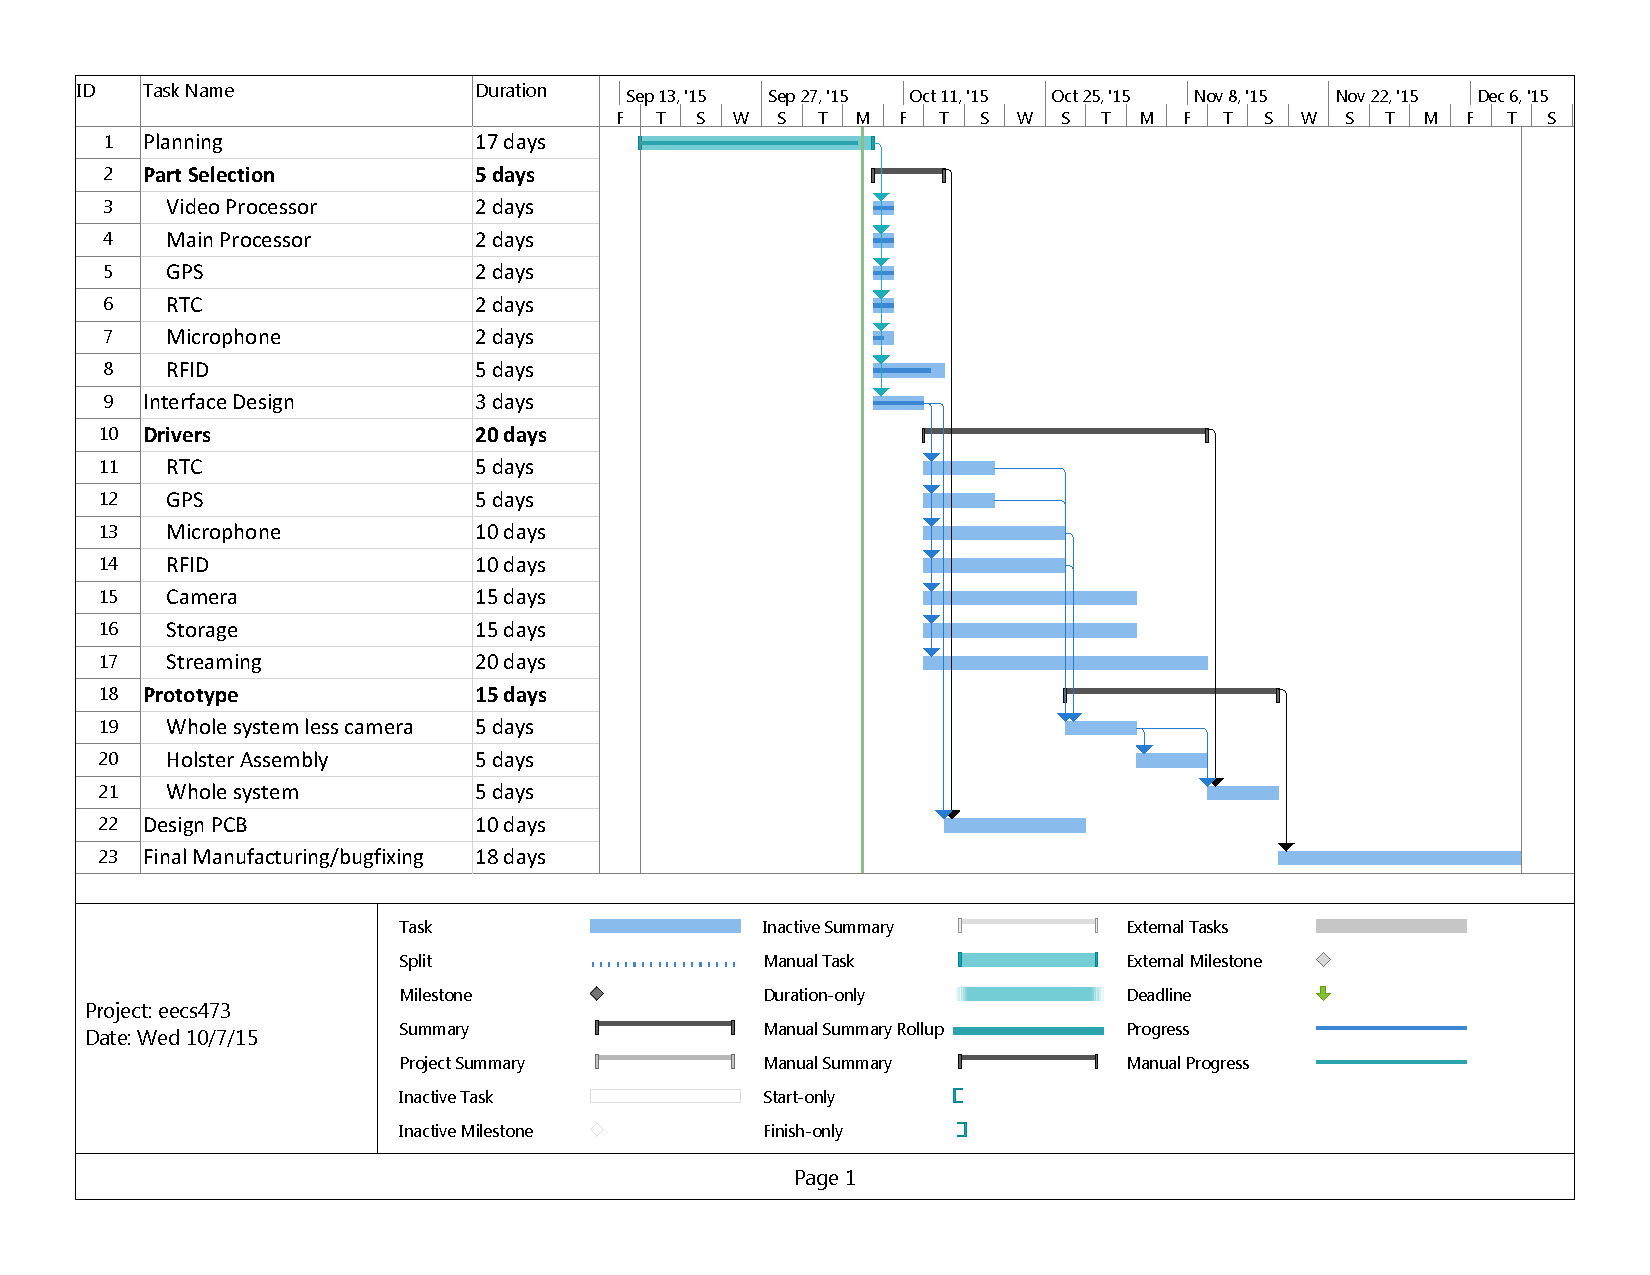
\includegraphics[width=1.1\textwidth]{gantt}
        \caption{Gantt chart}
        \label{fig:gantt}
    \end{figure}
\end{landscape}

\newpage

\section{Software Interfaces}
\label{app:software_interfaces}

\subsection{UVC/Camera Interface}
\lstinputlisting{uvc.h}

\newpage

\subsection{Network Interface}
\lstinputlisting{network.h}

\newpage

\subsection{GPS Interface}
\lstinputlisting{gps.h}

\newpage

\subsection{Trigger Interface}
\lstinputlisting{trigger.h}

\newpage

\section{PCB Design and Layout}

\begin{figure}[h]
    \centering
    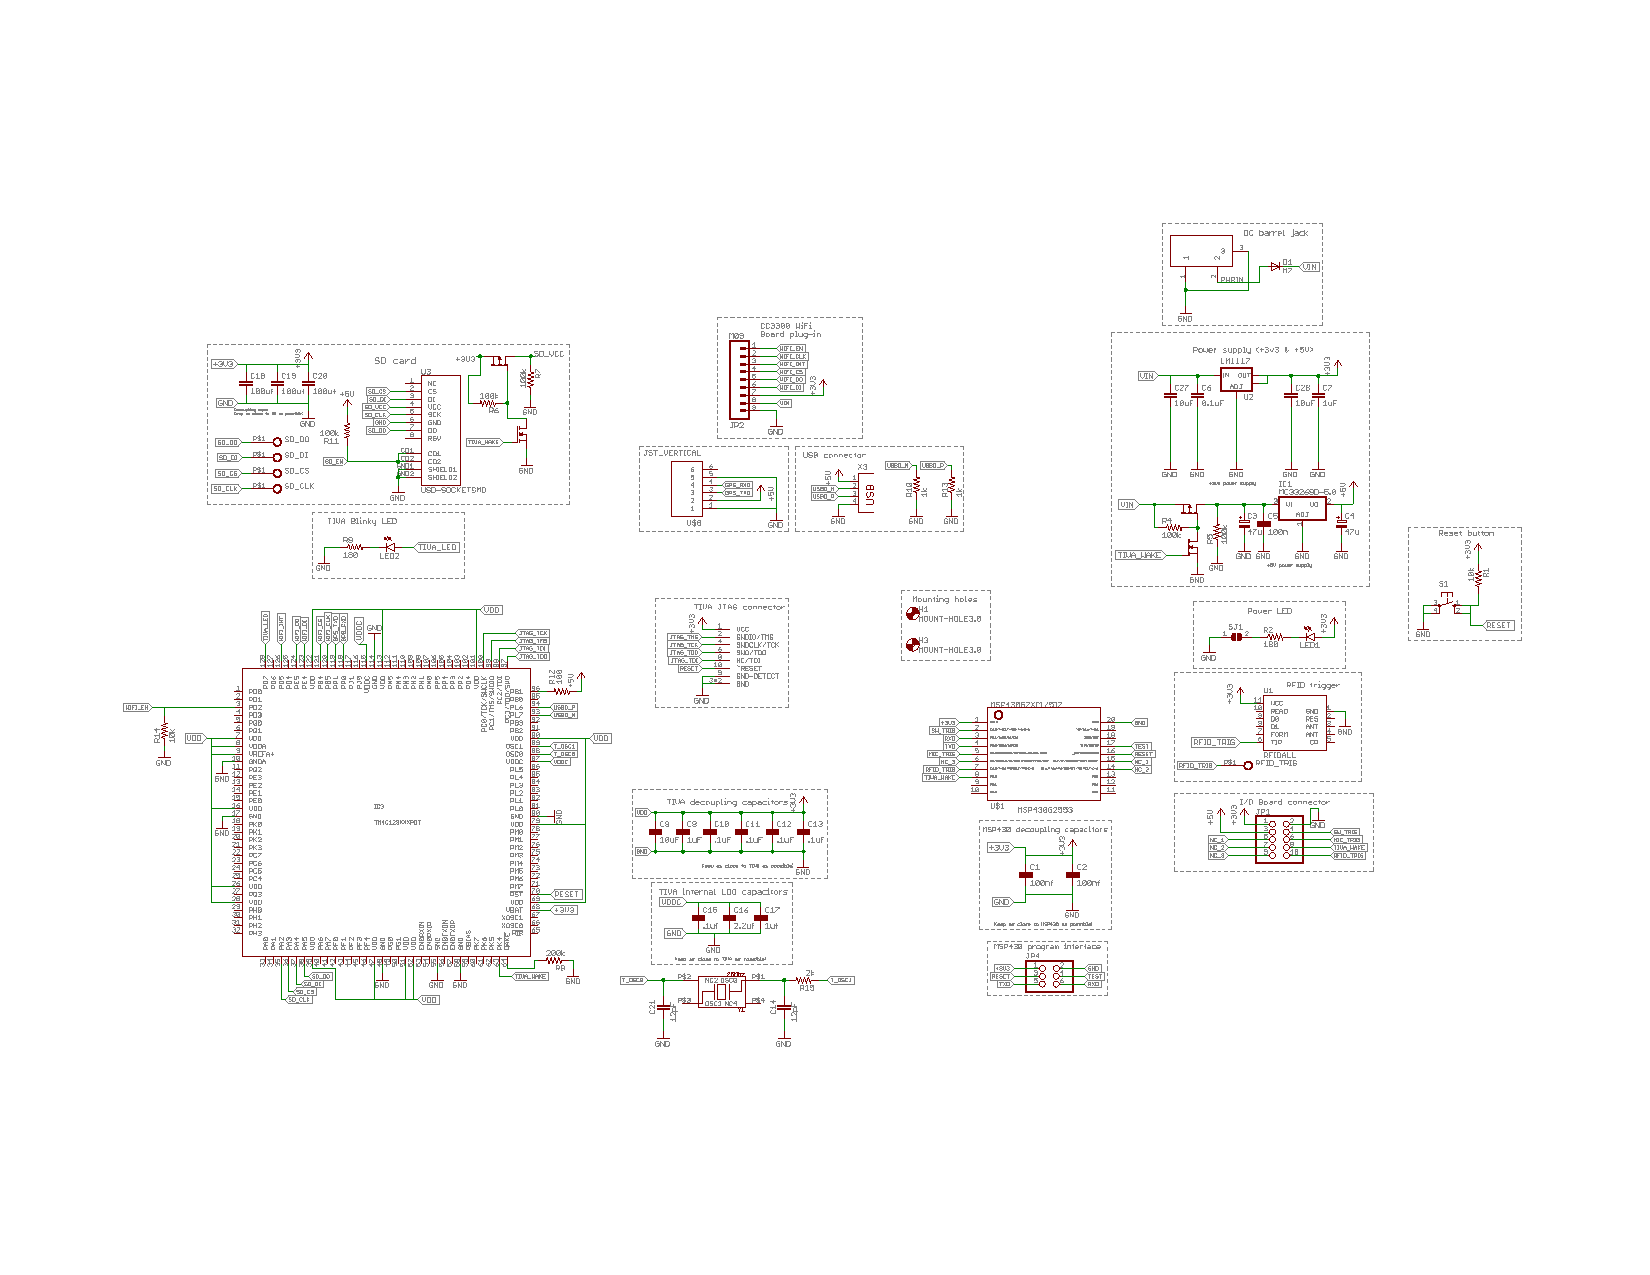
\includegraphics[angle=-90,width=0.75\textwidth]{BodyCamBoard_sch}
    \caption{Main board schematic}
\end{figure}

\begin{figure}[h]
    \centering
    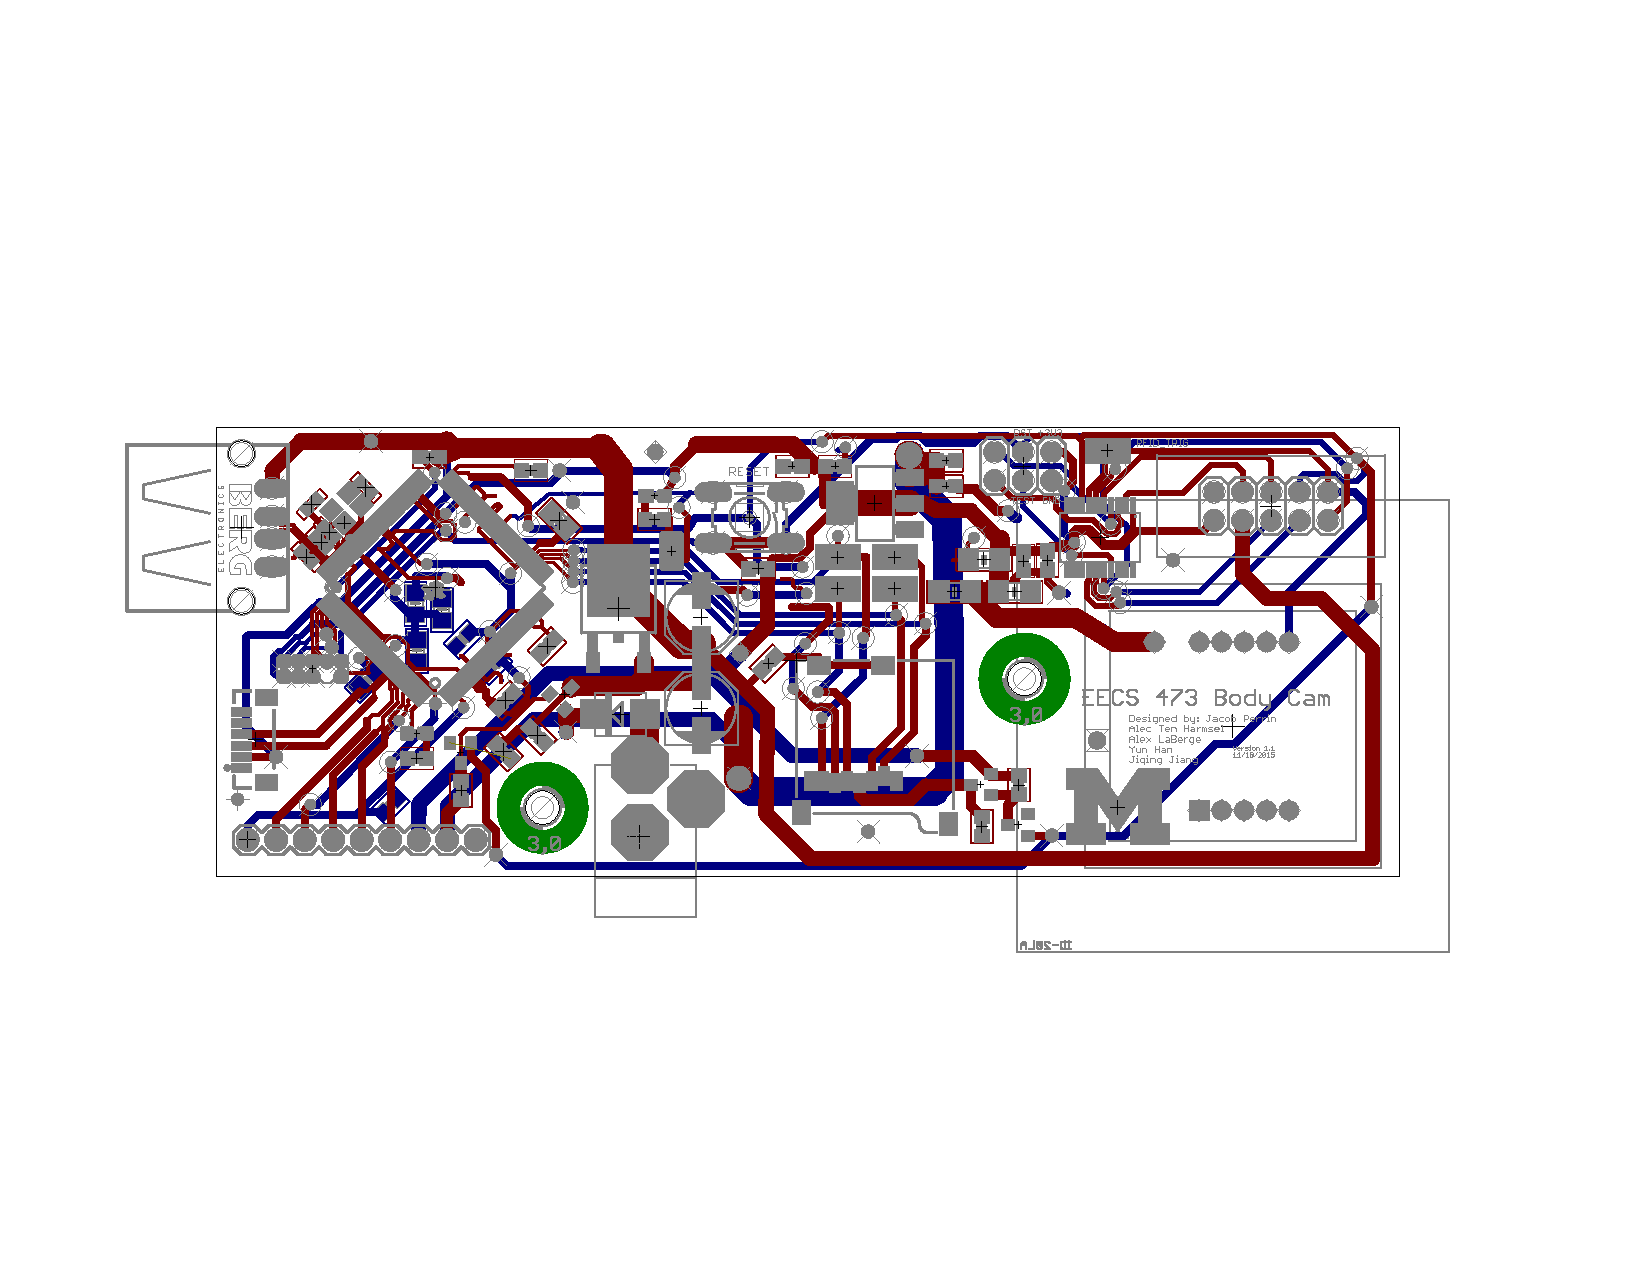
\includegraphics[angle=-90,width=0.99\textwidth]{BodyCamBoard_brd}
    \caption{Main board layout}
\end{figure}

\begin{figure}[h]
    \centering
    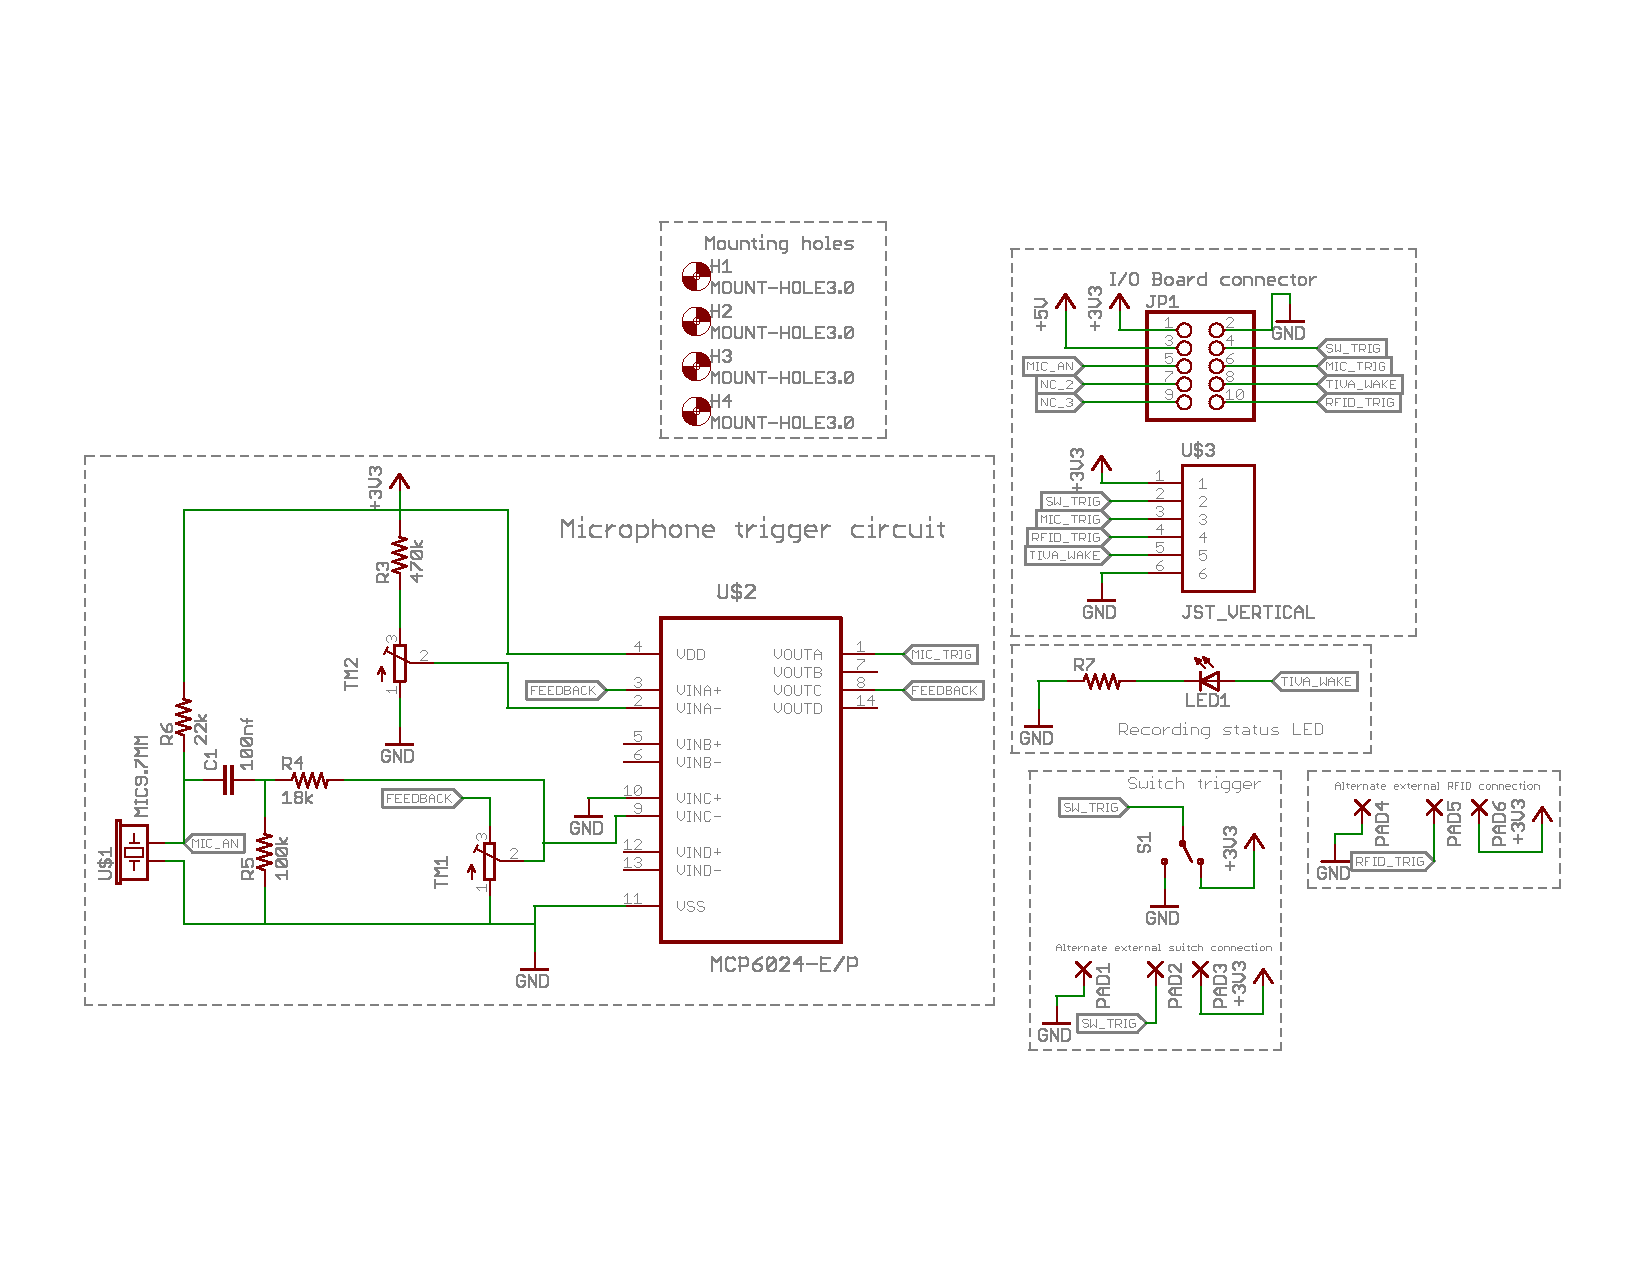
\includegraphics[angle=-90,width=0.99\textwidth]{IOBoard_sch}
    \caption{I/O board schematic}
\end{figure}

\begin{figure}[h]
    \centering
    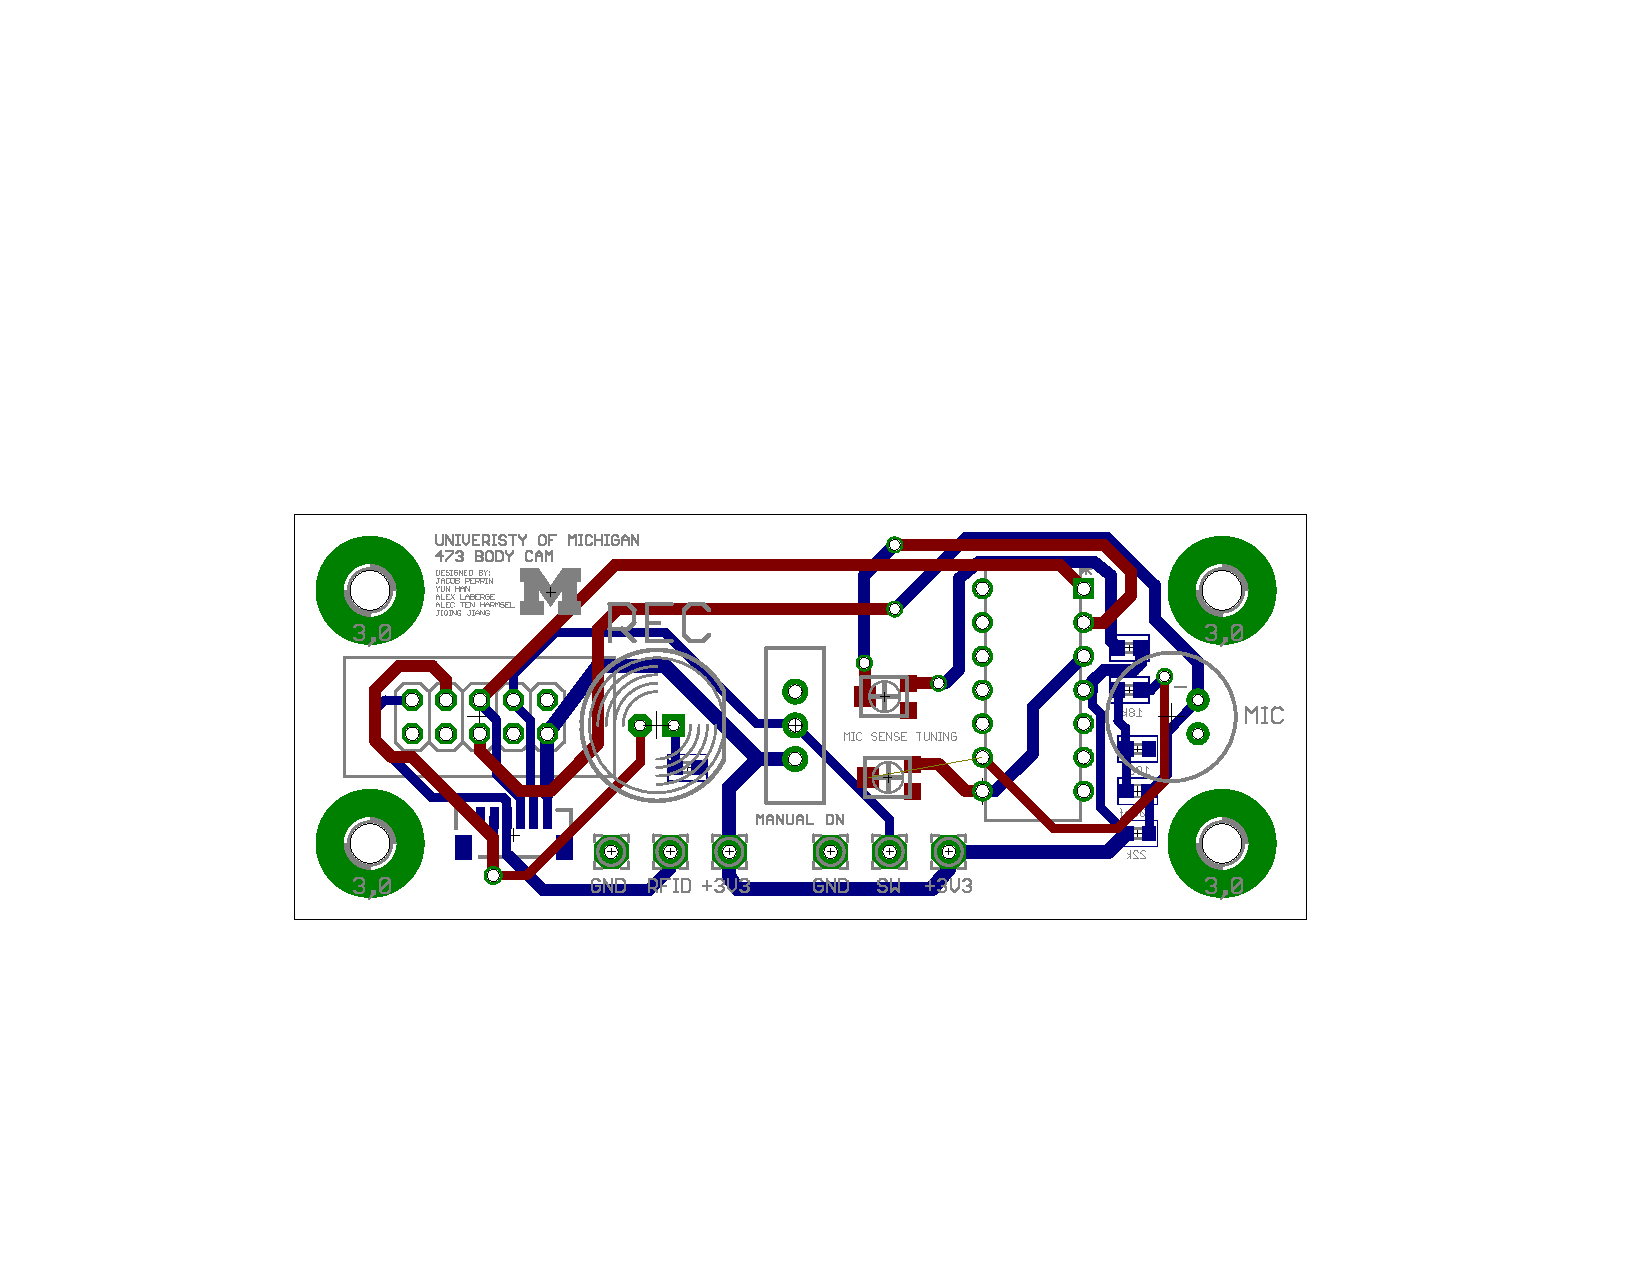
\includegraphics[angle=-90,width=0.99\textwidth]{IOBoard_brd}
    \caption{I/O board layout}
\end{figure}

\end{document}
